\chapter{Outbreeding Systems}
\label{cha:Lush_Chapter_26}
\index{Crossbreeding|(}
\index{Heterosis}
\index{Outbreeding|(}

Outbreeding is the general scientific term for mating animals distinctly
less closely related to each other than the average of the population
concerned. Its general effects are the opposite of those of inbreeding.
Outbreeding increases the heterozygosity of the individual and
increases the uniformity of the breed when it is first practiced, although
in a generation or two it comes to a limit in these respects. Continued
outbreeding merely serves to hold this individual heterozygosity and
breed uniformity. Any families which may have started to separate from
the rest of the breed are blended again toward the breed average by
crossing them with each other.

The practical usefulness of outbreeding rests on the general fact
that favorable effects of genes are apt to be dominant over the unfavorable
ones. Therefore, outbreeding increases the average individual
merit of the animals but lowers the breeding values of the best among
them. It increases at first the uniformity of the breed, but hampers further
progress in breed improvement. This superiority of the outbred
animals over the average of their parents in individual merit is so general
a phenomenon in many kinds of plants and animals that it has
been called ``hybrid vigor'' or ``heterosis.'' It is not often extreme unless
the parents are from different inbred lines or have in some other way
been made distinctly different from each other in the genes they carry.
The maximum practical usefulness of outbreeding systems is in the
production of market animals or purebred animals which are to be
shown to advertise the herd but which are not intended for breeding
use.

\section*{CROSSBREEDING}

Crossbreeding is the mating of two animals which are both purebred
but belong to different breeds. The mating of a purebred sire of
one breed to high grade females of another is often included under the
term crossbreeding.

Crossbreeding is often practiced in producing swine, sometimes in
producing poultry, and in some regions is extensively practiced by
sheepmen. Thus, in the northwestern range states many sheepmen plan
to keep one-quarter to one-half Merino or Rambouillet blood in the
ewes but use mutton rams on these ewes to produce market lambs.
Crossbreeding is rarer with cattle and horses; but there are certain
well-established practices of it, such as the production of blue-gray cattle for
feeding by crossing Angus and white Shorthorns, or the practice of certain
ranches --- e.g., the {SMS} ranch near Stamford, Texas --- in maintaining
an undercurrent of Shorthorn blood but of using bulls in the ratio
of 90 Herefords to 10 Shorthorns. Crossbreeding among cattle is also
practiced on a commercial basis along the Gulf coast, where many cattlemen
try to keep a quarter to a half Brahman blood in the cow herd,
but for siring the market steers and heifers use bulls from the beef
breeds which originated in Europe.

There have been many crossbreeding experiments with sheep, but
most of those have been planned to find what kind of ram is most profitable
for use upon range-bred ewes carrying a considerable amount of
Merino or Rambouillet blood. There have been several crossbreeding
experiments with swine to find how much general advantage there
might be in such crossing. The few crossbreeding experiments which
have been conducted with cattle have been directed mainly toward a
genetic analysis of the difference between breeds rather than toward
finding whether crossbreeding is a commercially successful practice.

Crossbreeding, like any other form of outbreeding, tends to lower
the breeding value of the individual by making it more heterozygous
and by making selection among the crossbred individuals less effective.
Like other forms of outbreeding it promotes individual merit because
of general dominance of genes favorable to size, vigor, fertility, etc.

When the crossbreds are used for breeding purposes, their offspring
are more variable than the crossbreds were and generally average
somewhat lower in individual merit. If both parents are crossbreds, the
offspring usually average below their purebred grandparents in individual
merit. Often the distribution of the offspring of crossbreds is
distinctly skewed, there being few which exceed the average of the crossbreds
and many which fall below it -- some of them far below.\footnote{Besides
the general dominance of favorable effects, it is probable that much of
this asymmetry in the distribution of the offspring of crossbreds is caused by gene
interactions such as those studied by Rasmusson (1933, \textit{Hereditas}, 18:245--61). In
more general terms it can be pictured as shown in Figures~\ref{fig:Lush_Figure_20}
\ref{fig:Lush_Figure_21}. The pure breeds crossed will usually have been in different
peaks, each more desirable than the adjacent genotypes. A general tendency to dominance
of the favorable effects of genes may keep the crossbreds high in individual merit. But
when the crossbreds reproduce, many of their offspring will fail to get some of the
genes vital for the successful functioning of the complete sets of genes which came
to the crossbreds from each of their purebred parents. Many of the offspring of the
crossbreds will, therefore, fall into some of the intervening valleys of low merit.}
But if one is to make full use of the heterosis of the crossbred females, it may
be necessary to use them for breeding. For example, in swine the number
of pigs farrowed and weaned and their weight at birth and probably
also at weaning are perhaps more dependent on the dam's characteristics
as a mother and nurse than on the genes which the pigs themselves
have, although the latter certainly play a part. It will be necessary to use
the crossbred females for breeding if this part of their heterosis is to be
used. Similar consideration would apply to egg production in poultry
and milk production in dairy cows. Some swine producers attempt to
solve this by keeping the crossbred gilts for breeding purposes and
breeding them to a purebred boar of a third breed. If all three breeds
nick well with each other in crosses, the pigs from such a ``triple cross''\index{Triple crossing}
should show many of the advantages of the original crossbreds besides
permitting their dams to show the effects of heterosis on their fecundity
and nursing ability. The triple-cross pigs are usually more variable,
since their crossbred dams transmit various combinations of genes to
them. The breeds can be chosen so that the triple-cross pigs will be as
uniform in color as the first-cross pigs. This is done by choosing for the
third cross a boar of a breed which has a conspicuous and dominant
color, such as solid white. This practice might theoretically be continued
to a fourth or even a fifth cross with only a little loss of heterosis in
the dams, but it becomes increasingly difficult to find more breeds which
are distinct from those already used and yet which nick well with all of
them. Actually this practice is rarely carried past the triple-cross.

\index{Crisscrossing|(}
``Criss-crossing'' is another method proposed\footnote{1935, Minnesota Agr.
Exp. Sta., Bul. 320.} for utilizing heterosis in the dams but not incurring
the full decline in average individual merit which usually occurs when
crossbreds are mated together. The plan is to use purebred sires all the time
but to alternate breeds. Thus, sows produced by crossing breeds \textit{A}
and \textit{B} would be mated back to \textit{A}. Their daughters (carrying
75 per cent of \textit{A} blood) would be mated to a \textit{B} boar. The
gilts thus produced (carrying 37\nicefrac{1}{2} per cent of \textit{A} blood)
would then be mated to an \textit{A} boar. If this were practiced regularly,
it would approach the condition in which each crop of pigs had \nicefrac{1}{3}
of its inheritance from one breed and \nicefrac{2}{3} from the other, but all
the sires used would be purebreds. The Minnesota Station reports good results
from this system, as far as it was carried in six years of experimenting. Some
practical difficulties with overlapping of generations are to be expected in
herds where only one boar is kept and is used both on gilts and on older sows.
This would not occur where all the sows are the same age. Figure 45 shows
examples of how pedigrees would appear after several generations of regular
criss-crossing or three-breed crossing.

\begin{figure}
	\centering
    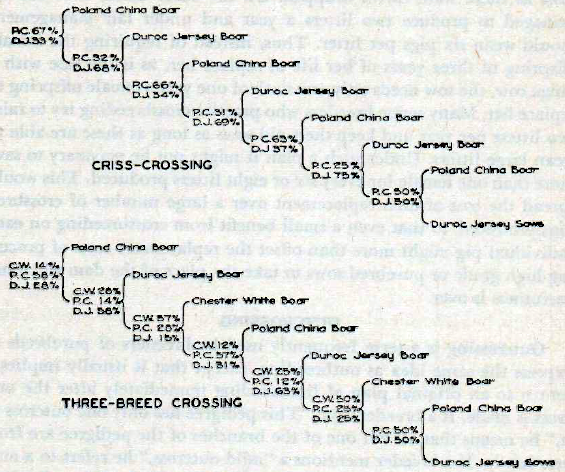
\includegraphics[width=\textwidth]{Figure_45.png}
    \caption{Illustrative pedigrees of ``criss-crossed'' and ``three-breed crossed'' pigs.}
    \label{fig:Lush_Figure_45}
\end{figure}
\index{Crisscrossing|)}

Whether crossbreeding is a sound commercial policy depends on
the balance between the extra size, vigor, fertility, etc., which is usually
gained by crossbreeding and the extra cost of replacement which is
incurred when the crossbred parents are replaced. Heterosis does not
occur uniformly in all crosses. That is, not all breeds nor all animals
within the same breed ``nick'' equally well. The heterosis from crossing
breeds of farm animals is not apt to be larger than around 2 to 8 per
cent increase over the average of the parental breeds for such things as
size, growth rates, fertility, or other complex physiological traits. It is
generally largest for vitality as measured by percentage raised of those
born. There is nothing in animal breeding to correspond to the very
large amount of heterosis which the corn breeders often find when they
cross two inbred lines. Presumably the underlying principles are the
same, but nothing corresponding closely to the inbred lines of corn
exists in the breeds of farm animals.

Crossbreeding is most likely to be profitable where fertility is highest
and the percentage of replacements necessary to keep up the female
herd is lowest. For example, with cattle under most range conditions 70
calves weaned per 100 cows per year is considered a good calf crop. With
half the calves being females, a herd would need to be kept three years
in order to produce enough females to replace the original cows even if
all heifer calves which lived to weaning time were used without selection.
If the average cow only stays in the herd about six to eight years,
nearly half of all her daughters will be needed to maintain the number.
If crossbreeding were practiced and all calves were sold for beef, this
would necessitate an annual replacement of about one-fourth as many
cows as there were calves dropped. On the other hand, sows can be
managed to produce two litters a year and under fair management
should wean six pigs per litter. Thus, instead of requiring the female
offspring of three years of her life to replace her, as is the case with a
range cow, the sow needs only one-sixth of one year's female offspring to
replace her. Many swine breeders who practice crossbreeding try to raise
two litters per year and keep their old sows as long as these are able to
wean large litters. Under such a plan it might not be necessary to save
more than one female for every six or eight litters produced. This would
spread the cost of each replacement over a large number of crossbred
pigs produced, so that even a small benefit from crossbreeding on each
individual pig might more than offset the replacement costs of procuring
high grade or purebred sows to take the place of the dam when her
usefulness is over.
\index{Crossbreeding|)}

\section*{OUTCROSSING}
\index{Outcross|(}

Outcrossing is a term frequently used by breeders of purebreds to
express the same idea as outbreeding, except that it usually implies a
return to an original plan of linebreeding immediately after the outcross
is made. If a breeder says: ``This pedigree has only one outcross in
it,'' he means that all but one of the branches of the pedigree are from
one family. If a breeder mentions a ``mild outcross,'' he refers to a mating
with an animal which is not quite of the family he is breeding but
which is related to it. A man after having practiced linebreeding for a
time may say that he needs an outcross. In this case he means that he
needs to mate his stock to animals from some other line; but the usual
implication is that, after one generation of outbreeding, he will return
to using animals of his original family, attempting by selection to hold
the good traits introduced by the outcross, while by linebreeding to his
chosen family again he tries to recapture and hold all the good traits he
already had in that family. The corn breeders call this kind of a process
``convergent improvement'' when used on their more intensely inbred
material.

Outcrossing is a minor part but eventually a necessary part of most
linebreeding programs. Any linebreeding which is carried far is apt to
fix some undesired traits so that mild outcrossing may be necessary to
remedy them. If the outcross is a success, the breeder is sometimes so
carried away by enthusiasm for it that he gives up his plan of returning
to his original family and decides to mate the outcrossed animals together.
To do this is the same in principle, although less extreme in degree,
as attempting to fix desired crossbred traits by breeding crossbred
females to crossbred males.
\index{Outcross|)}

\section*{BACKCROSSING}
\index{Backcrossing}

Backcrossing is the mating of a crossbred animal back to one of the
pure parent races which were crossed to produce it. It is a term commonly
used in genetic studies but not widely used by breeders. In
genetic analyses, particularly where one of the parents possesses all or
most of the recessive traits, the backcross permits a surer analysis of the
genetic situation than an $F_2$ generation does. General experience with
backcrosses in practical animal breeding has not been quite as satisfactory
as experience with crossbreds. The backcrosses retain some of the
heterosis in many cases, but rarely as much as the first crosses or the
triple crosses.

\section*{TOPCROSSING}
\index{Topcrossing}

Topcross usually refers to the last sire in a pedigree. When a breeder
mentions a ``Scotch-topped'' Shorthorn, he means a purebred Shorthorn
whose dam belongs to a family not originating in Scotland but whose
sire and perhaps maternal grandsire were ``straight Scotch.'' When a
breeder says that ``this animal has four topcrosses of Scotch blood,'' he
means that it is by a Scotch sire, that its dam is by a Scotch sire, that its
maternal grandam is by a Scotch sire and that the dam of the maternal
grandam is by a Scotch sire. Presumably the pedigree farther back in the
maternal line is not Scotch.

Top crossing is the same in principle as grading, except that topcrossing
is usually applied to different families within a pure breed,
whereas grading is applied to the continued use of sires of one pure
breed starting with foundation females which were of another breed or
of no particular breed at all.

In plant breeding topcrossing is sometimes used to mean the production
of seed by putting pollen from an inbred sire on plants from a
good commercial variety.

\section*{GRADING}
\index{Grading|(}

When the pure breeds were new and relatively scarce in this country,
grading common or mongrel stock up to the purebred level by the
continued use of sires of a pure breed was the quickest way available for
improving commercial herds. Many of the experiment stations conducted
experiments or demonstrations in the results of such grading.
Generally the first cross showed a marked improvement over the original
stock. The further improvement made by each successive cross was
progressively less. Grading can rapidly bring the stock near the level
of the pure breed which is being used for the grading. Grading will
remain the most important form of breeding for the commercial market
as long as the merit of the pure breeds is distinctly above that of
the commercial herds, and unless heterosis itself is so important that
wider out breeding plans, such as criss-crossing, are more profitable than
continued grading to one pure breed. The fact that in so many grading
experiments the major improvement has come in the first cross seems to
indicate that some of the improvement in the first cross was from heterosis.
No doubt the original mongrels in such experiments had at least
a few desirable genes which should have been kept if there had been any
way to select them and keep them while letting the rest of the genes
from the mongrels be bred out by the continued grading.
\index{Grading|)}

\section*{SPECIES HYBRIDS}
\index{Species!crosses|(}

The mule is the only commercially important species hybrid in
North American animal husbandry. Male mules are always sterile as far
as is yet known. A few well-authenticated cases of fertile mare mules
have been reported,\footnote{For two examples, see \textit{Jour. of
Heredity} 19:412--16, 1928.} but these have been so rare that they have
had no commercial importance. These fertile mare mules might possibly be
the means of transferring some characteristics from the ass species to the
horse species or the reverse. Because mules are sterile the problems of
mule breeding are only those of choosing the most suitable kinds or
breeds of mares and of jacks for crossing. The reciprocal cross, called a
``hinny,'' has been made many times, but is generally regarded as inferior
to the mule as a work animal.

Crosses between zebu cattle and cattle breeds of European origin
are of considerable economic importance in the Gulf coast region of the
United States and in nearly all the tropical regions of the world. Some
would regard these as species crosses, but the majority opinion is that
zebus and the cattle of European origin are not distinct species.
Intermediate types exist in the regions between their native lands, as in
southeastern Europe, Asia Minor, southern Siberia, and the northeastern
regions of Africa.

Crosses between European cattle and the American bison have been
made. Some would regard this as a generic cross. The males are sterile,
but many of the females are fertile. By backcrossing these females to
cattle and to bison, attempts to form a new breed, the ``cattalo,'' have
been made on a fairly large scale, but commercial success was not
achieved.

Other species crosses which involve farm animals but have hardly
passed the stage of zoological curiosities or menagerie specimens
include: horse and zebra, European cattle and yak, American bison and
yak, American bison and European bison or wisent, yak and zebu,
mouflon and domesticated sheep, bactrian and dromedary camels,
chicken and guinea hen, pheasant and hen, and peacock and hen.
Hybrids between yaks and other cattle are economically important in
some parts of China. Crosses between sheep and goats may start to
develop, but the embryos die and are resorbed or aborted long before
the normal gestation period is completed. A similar fate happens to the
embryos from crosses of chickens and turkeys.

Species hybrids do not seem to offer as much opportunity for economic
improvement in animal breeding as they do in plant breeding.
\index{Species!crosses|)}

\section*{SUMMARY}

Outbreeding generally leads to individual excellence but low breeding
worth.

Outbreeding systems hamper progress in further improvement of a
breed because they destroy families by constantly crossing together any
which start to develop. They thus make the breed temporarily more
uniform than if outbreeding were not practiced.

Crossbreeding is a special form of outbreeding where the parents
belong to different breeds. It generally results in increased size, vitality
and fertility; but the amount of this increase is variable in different
crosses. The economy of crossbreeding depends upon whether the
increase in these things is more than enough to balance the possible
confusion and increase in cost of replacements under a crossbreeding
system.

Crossbreeding is more apt to be profitable where fertility is highest
and females can be kept for the longest period of time and where the
cost of their replacement is lowest. Mainly for these reasons crossbreeding
is practiced most widely with swine and poultry and next with
sheep.

Outcrossing usually applies only to matings within a pure breed. It
may mean the same thing as outbreeding but usually implies also an
intention to return to the original family or strain after making the one
outbreeding mating.

Backcrossing is mating a crossbred animal back to the same kind of
animal as one or the other of its parents.

Topcross refers to the sire, maternal grandsire, and sires of the other
females in the purely maternal line. Generally it is used only within
pure breeds.

Grading is the continued use generation after generation of males
of one pure breed on an original foundation of another breed or of no
particular breed. Grading is the most economical way of lifting the
commercial stock rapidly toward the level of the purebreds.

\section*{REFERENCES}

For recent reports on experiments with crossbreeding, see the following
bulletins from agricultural experiment stations: Arkansas 411,
California 598, Iowa 380, Minnesota 320, Mississippi 347, Nevada 153,
Pennsylvania 279, and Wyoming 210. See also articles in \textit{Journal of
Animal Science} 1:213--20, and \textit{Scientific Agriculture} 16:322--36 and
19:177--98. Also see mimeographed leaflet BDIM-Inf. 30, May 1946,
from the USDA.
\index{Outbreeding|)}